\chapter{Introdução}
\label{cap:introducao}
% --------------------------------------------------------------------------

A democratização do acesso à órbita baixa terrestre (\textit{Low Earth Orbit} -- LEO), impulsionada pela padronização da arquitetura \textit{CubeSat Design Specification} (CALIFORNIA POLYTECHNIC STATE UNIVERSITY, 2022), viabilizou a execução de experimentos científicos e tecnológicas por universidades e centros de pesquisa a custos substancialmente inferiores aos das missões espaciais tradicionais. No entanto, a padronização de volume e massa inerente a essa classe de nanossatélites, ilustrada pelo arranjo estrutural do nanossatélite universitário brasileiro ITASAT-1 na Figura~\ref{fig:itasat}, impõe severas restrições mecânicas. Durante as etapas de ascensão no veículo lançador e na ejeção orbital, o chassi primário do nanossatélite é submetido a um ambiente mecânico dinâmico severo, governado por normas internacionais rigorosas, como o \textit{General Environmental Verification Standard} (GEVS) (NASA, 2013). As diretrizes da Agência Espacial Brasileira (AEB, 2026) preconizam que a integridade estrutural do satélite e a proteção dos subsistemas de bordo exigem frequências naturais fundamentais elevadas ($f_1 \ge \SI{100.0}{\hertz}$), de modo a prevenir a ocorrência de ressonância com os modos acústicos e de baixa frequência do foguete.

\begin{figure}[htb]
  \caption{Arranjo estrutural e distribuição de subsistemas do nanossatélite universitário ITASAT-1}
  \label{fig:itasat}
  \begin{center}
    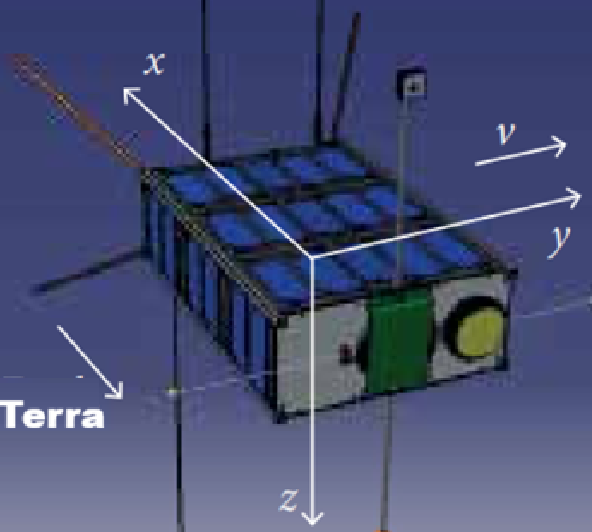
\includegraphics[width=0.75\textwidth]{figuras/itasat1_estrutura.png}
  \end{center}
  \fonte{Adaptado de Carrara \textit{et al.} (2017).}
\end{figure}

Investigações dinâmicas conduzidas em projetos nacionais como o nanossatélite SPORT (SANTOS \textit{et al.}, 2020), desenvolvido conjuntamente pelo Instituto Tecnológico de Aeronáutica (ITA), pelo Instituto Nacional de Pesquisas Espaciais (INPE) e pela NASA, evidenciam que a interface física entre o nanossatélite e o casulo lançador constitui a fonte primária de excitação vibratória e transitória de choque. Concebido com base no padrão operacional do \textit{Poly-Picosatellite Orbital Deployer} (P-POD) (PUIG-SUARI \textit{et al.}, 2002), o mecanismo cinemático de ejeção utiliza a expansão de uma mola principal para impulsionar o satélite ao longo de trilhos de deslizamento, conforme esquematizado na Figura~\ref{fig:interface}. Esse sistema opera sob regime de atrito seco e contato direto metal-metal entre os trilhos do satélite e o interior do tubo lançador. Por exigência normativa estrita da especificação CubeSat, os quatro trilhos longitudinais de \rail{} devem permanecer monolíticos, contínuos e dotados de rugosidade superficial controlada ($Ra \le \SI{1.6}{\micro\metre}$), impedindo qualquer descontinuidade geométrica externa que possa induzir travamento mecânico (\textit{jamming}). Em virtude dessa restrição de contorno fixa, qualquer estratégia de alívio de massa e de isolamento dinâmico passivo deve ser concentrada estritamente nos painéis estruturais internos do chassi.

\begin{figure}[htb]
  \caption{Interface mecânica e cinemática de contato entre os trilhos do CubeSat e o dispensador orbital P-POD durante o curso de ejeção}
  \label{fig:interface}
  \begin{center}
    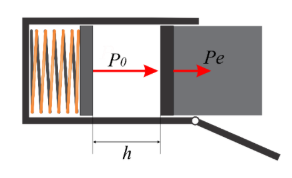
\includegraphics[width=0.65\textwidth]{figuras/interface_cubesat_deployer.png}
  \end{center}
  \fonte{Adaptado de Santos \textit{et al.} (2020).}
\end{figure}

Tradicionalmente, os chassis da classe CubeSat são usinados a partir de blocos maciços de ligas de alumínio aeroespacial, como o Al 6061-T6. Embora apresentem propriedades estáticas consolidadas, tais estruturas contínuas exibem acoplamento dinâmico rígido direto e reduzida capacidade de filtragem mecânica de frequências operacionais, transferindo quase integralmente a densidade espectral de potência (PSD) de vibração aleatória da base para as placas eletrônicas e cargas úteis sensíveis (SLEJKO \textit{et al.}, 2023). Como alternativa a esse gargalo físico, pesquisas recentes na fronteira da mecânica dos sólidos apontam para o uso de metamateriais celulares auxéticos com coeficiente de Poisson negativo ($\nu < 0$) (LI \textit{et al.}, 2026). Geometrias reentrantes, quando submetidas a solicitações mecânicas dinâmicas, exibem rotação controlada de costelas oblíquas e contração lateral sob tração (ou expansão lateral sob compressão), conferindo elevada Absorção Específica de Energia (\textit{Specific Energy Absorption} -- SEA), resiliência a impactos e formação de zonas proibidas de propagação de ondas elásticas (\textit{phononic bandgaps}) por interferência destrutiva e desacoplamento de impedância acústica (CUI \textit{et al.}, 2025; FARSHBAF \textit{et al.}, 2025). Tais propriedades tornam as treliças auxéticas candidatas ideais para atuarem simultaneamente como elemento estrutural resistente e como filtro passa-faixa/passa-baixa elastodinâmico passivo.

A viabilidade de manufatura dessas geometrias celulares complexas decorre do avanço da Manufatura Aditiva por Fusão em Leito de Pó a Laser (\textit{Laser Powder Bed Fusion} -- L-PBF), governada pelos preceitos de \textit{Design for Additive Manufacturing} (DfAM) (KHAN; RICCIO, 2024). Ensaios experimentais prévios demonstraram a aptidão de estruturas de suporte espacial manufaturadas aditivamente para resistir a perfis de qualificação aleatória GEVS sem falha estrutural (ROBERTS, 2018). Todavia, o dimensionamento e a otimização de matrizes celulares com modulação espacial de espessuras impõem barreiras computacionais críticas: a avaliação de uma única geometria por simulação tridimensional de Elementos Finitos (FEA) de alta fidelidade demanda tempos de processamento da ordem de minutos a horas, inviabilizando varreduras evolutivas com milhares de indivíduos. Para transpor esse custo proibitivo com rigor físico estrito, torna-se imprescindível a incorporação de Modelos Substitutos Neurais Guiados por Física (\textit{Physics-Guided Machine Learning}), fundamentados nas leis fenomenológicas de escala de Gibson e Ashby (1997), e orquestrados por uma máquina de estados finitos determinística em grafo de fluxo fortemente tipado (LangGraph) acoplada a algoritmos genéticos multiobjetivo (DEB \textit{et al.}, 2002).

Diante desse cenário, formula-se o problema central desta pesquisa: \textit{como parametrizar, acelerar e otimizar autonomamente a geometria de núcleos auxéticos reentrantes em liga AlSi10Mg fabricados por L-PBF, de modo a sintetizar um chassi primário CubeSat 1U que maximize a atenuação vibratória passiva para a carga útil e minimize a massa estrutural, satisfazendo simultaneamente os critérios normativos da norma NASA GSFC-STD-7000A, a integridade estática de escoamento e o limite de dano por fadiga estocástica de Steinberg?}

A hipótese que norteia este trabalho estabelece que a introdução de painéis auxéticos com ângulo de reentrância e espessura otimizados, combinada a arestas maciças funcionais de deslizamento, viabiliza uma redução de massa superior a \SI{50}{\percent} e uma atenuação na transmissibilidade dinâmica superior a \SI{10}{\decibel} em relação ao chassi monolítico convencional, mantendo a frequência fundamental acima de \SI{100.0}{\hertz} e o dano de fadiga aleatória dentro dos envelopes de segurança de voo.

O presente estudo delimita-se à resposta mecânica elastodinâmica em regime linear e à fadiga por vibração aleatória durante a fase de lançamento e ejeção em órbita baixa. A etapa de caracterização experimental com corpos de prova poliméricos em PLA (FDM) atua como prova de conceito dimensional, cinemática de montagem e validação preliminar do arcabouço numérico, enquanto a homologação estrutural da liga AlSi10Mg (L-PBF) é realizada computacionalmente em elementos finitos de alta fidelidade (\textit{FEA Ground Truth}) segundo a norma NASA GSFC-STD-7000A, estabelecendo os requisitos para a certificação física final em mesa vibratória. Aspectos relativos ao acoplamento termovácuo orbital (TVAC) e à degradação superficial por oxigênio atômico não integram o escopo experimental primário, sendo recomendados como extensões de trabalhos futuros.

Para desenvolver essa investigação de forma sistemática, a monografia está estruturada em seis capítulos. O Capítulo~\ref{cap:objetivos} formaliza os objetivos geral e específicos. O Capítulo~\ref{cap:revisao} apresenta a fundamentação teórica em nanossatélites, dinâmica de lançamento, metamateriais auxéticos, DfAM e modelos substitutos neurais informados pela física. O Capítulo~\ref{cap:metodologia} descreve detalhadamente o método de modelagem, o banco de dados FEA, a formulação da rede neural residual e o fluxo multiagente. O Capítulo~\ref{cap:resultados} discute a fronteira de Pareto NSGA-II, a decisão multicritério TOPSIS, a validação física de alta ordem e o confronto direto com o chassi convencional de referência. Por fim, o Capítulo~\ref{cap:conclusao} sintetiza as principais contribuições técnicas e delineia os passos para futuros testes em mesa vibratória e qualificação de voo.
